\chapter{Application}
\label{chap:application}
The GNN model introduced in \autoref{chap:gnn} will be benchmarked on various datasets in the following sections. All reference data was calculated using the 6-31G(2df,p) basis at theory level B3LYP. 

Models will be evaluated by their iteration count until convergence, by the energy difference from the converged solution the DIIS error (see \autoref{eq:diis_error}), and by the RMSE. The inference time of all models, just a few milliseconds, is roughly three orders of magnitude shorter than that of a typical DFT calculation, and can therefore be regarded as negligible. This performance holds across all applications discussed below.

\section{QM9 - \ch{C7H10O2} Isomers}
\label{sec:qm9_isomers_benchmark}
There are 6095 structural isomers of \ch{C7H10O2} in the QM9 dataset (see \autoref{sec:dataset}). Analogous to the trials performed in \autoref{sec:further_trials_mlp}, we will train and validate on a randomly drawn sample of 500 isomers\footnote{using \textsc{scf\_guess\_datasets} (see \autoref{subsec:gnn_normalization})}. This reduction is necessary to make training and hyperparameter-tuning feasible in the scope of the thesis. Contrary to the full matrix prediction schemes of \autoref{chap:fock_matrix_predictions}, we employ sub-matrix predictions and reconstruct the full matrix, thus increasing the actual number of samples significantly. Per molecule, we obtain 7, 10 and 2 samples for \ch{C}, \ch{H} and \ch{O}, respectively, yielding a total of 3500 \ch{C}, 5000 \ch{H} and 1000 \ch{O} samples. This already provides a certain rotational variability, but additional rotations can be introduced through data augmentation during training to develop a model that is insensitive to rotation when predicting density.
\newpage
\subsection{Initial training}
\label{subsec:qm9_isomers_initial}
%! refer to MGNN_6-31G_NO_AUG_07_07_manual_ref.pth
To evaluate the performance of the GNN devised in \autoref{chap:gnn}, several manual runs were initiated during development, with hyperparameters set to the values listed in \autoref{tab:init_hparams}. 
\begin{table}[H]
    \centering
    \caption[Hyperparameters - initial MGNN training (manually selected)]{Hyperparameters used for the initial MGNN training (manually selected)}
    \label{tab:init_hparams}
    \begin{tabular}{ll ll}
        \toprule
        \textbf{Hyperparameter} & \textbf{Value} & \textbf{Hyperparameter} & \textbf{Value} \\
        \midrule
        Hidden dimension & 256 & Msg. passing rounds & 4 \\
        MsgNet layers & 3 & MsgNet dropout & 15 \% \\
        Batch size & 16 & Grace period & 10 epochs \\
        Target & Density matrix & Loss function & MSE (blockwise) \\
        Learn rate (initial) & $2.68 \times 10^{-3}$ & Weight decay & $1.78 \times 10^{-5}$ \\
        Edge threshold & 3 \AA & Data augmentation & No \\
        \midrule
        Learn rate factor & 0.5 & Learn rate patience & 3 epochs \\
        Learn rate threshold & $10^{-3}$ & Learn rate cooldown & 2 epochs \\
        Learn rate min & $10^{-6}$ & — & — \\
        \bottomrule
    \end{tabular}
\end{table}
Note that these initial runs didn't use data augmentation, so the training comprised 400 samples (80\% of our data), leaving 10\% for validation and 10\% for testing. The grace period (time without improvement) was set to 10 epochs to leave the learning rate scheduler sufficient time to take effect.\\

Training and validation losses both monotonically decrease until around epoch 30. As can be seen in \autoref{fig:initial_train_qm9_isomers}, while the loss on the validation set flattens out rather early, training loss decreases throughout the entire training process. 
\begin{figure}[H]
    \centering
    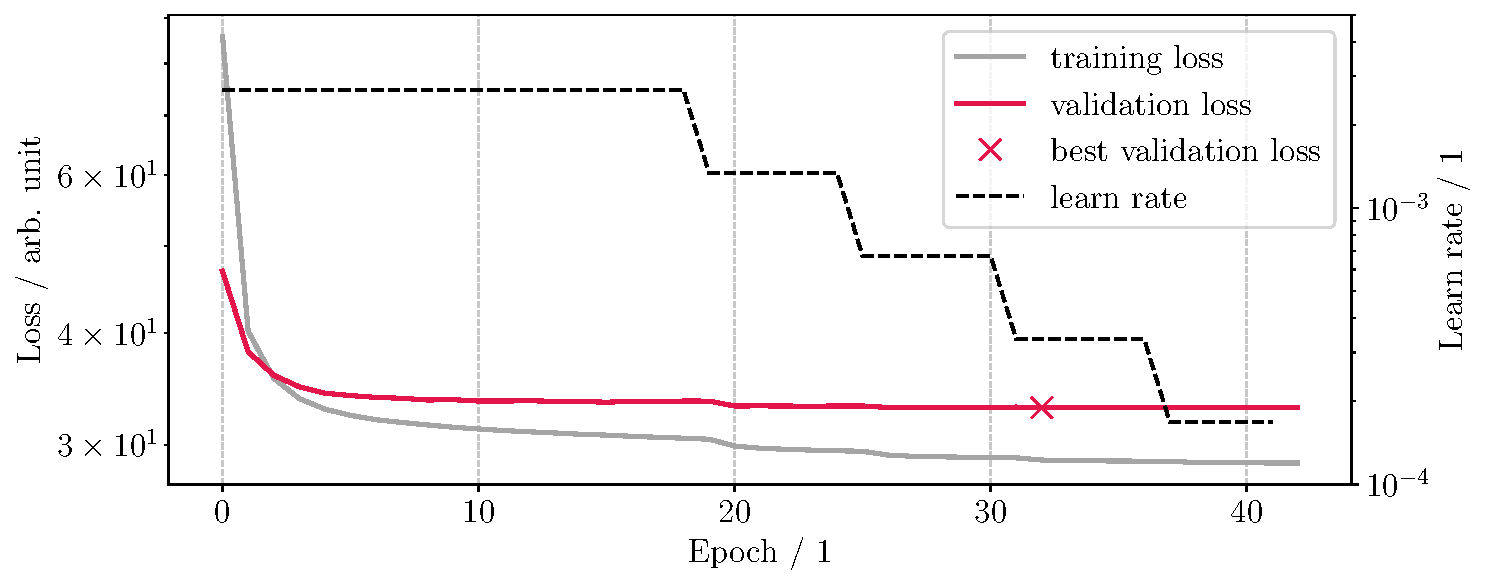
\includegraphics[width=0.75\textwidth]{../fig/gnn/MGNN_6-31G_NO_AUG_07_07_manual_ref_train_val_loss.pdf}
    \caption[Initial GNN loss on QM9-isomers]{Initial GNN training / validation loss and corresponding learn rate per epoch on QM9-isomers.}
    \label{fig:initial_train_qm9_isomers}
\end{figure}
Both losses are reduced further by stepwise decrease of the learn rate. This run produced the best model in epoch 33, with a validation loss of $33.00$ and a training loss of $28.83$, indicating slight overfitting which is to be expected especially without data augmentation in the training samples. The performance of the model $\text{GNN}_\text{initial}$ on the test set is compared to other models and the various guessing schemes in a summarizing \autoref{tab:qm9_isomers_test_overview} placed at the end of this chapter. 

\subsection{Hyperparameter tuning}
\label{subsec:qm9_isomers_hyperparamtuning}
Validation loss is used as a benchmark to select the best model from a hyperparameter run. While we will also prefer models with lower loss, we must be very careful not to select models which look good on paper but perform worse due to the lack of sufficient correlation between MSE and iteration count. For this reason, we will base our hyperparameter search on the $\text{GNN}_\text{initial}$ model and explore the hyperparameter space in a structured way. 

\textbf{Data augmentation}\\
$\text{GNN}_\text{initial}$ already performed quite well in terms of iterations without using any data augmentation. One might argue that there is already some data augmentation intrinsic to the training set due to the different orientations of atoms in various molecules. 
\begin{figure}[H]
    \centering
    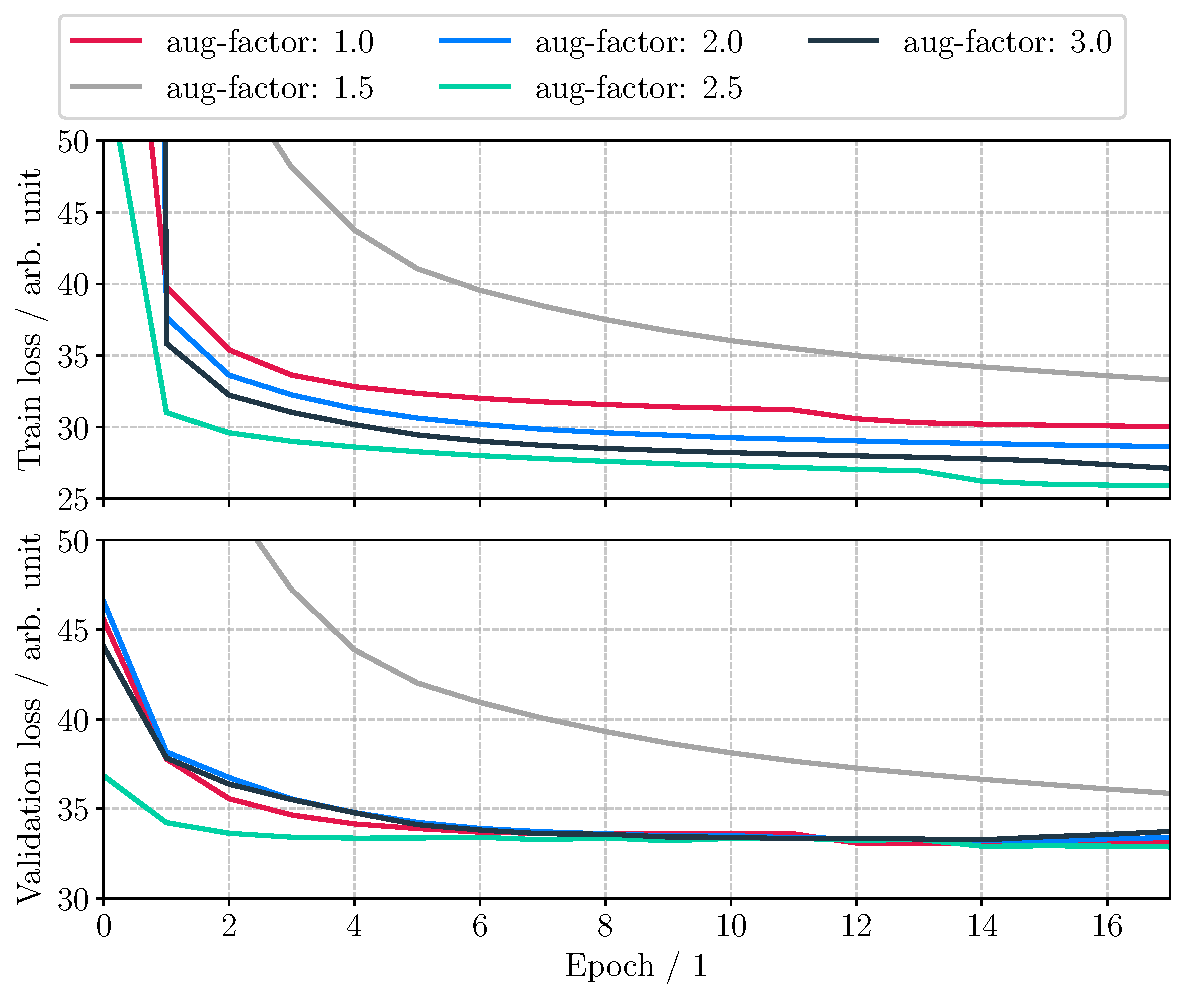
\includegraphics[width=0.75\textwidth]{../fig/application/aug_train_val_loss.pdf}
    \caption[GNN loss for different augmentation factors on QM9-isomers]{GNN loss for different data augmentation factors on QM9-isomers. All other hyperparameters are chosen as in \autoref{tab:init_hparams}.}
    \label{fig:loss_hyper_qm9_isomers}
\end{figure}
A comparison of the training and validation loss between different augmentation factors in \autoref{fig:loss_hyper_qm9_isomers} shows no clear trend regarding the choice of the augmentation factor. While a factor of $2.5$ initially outperforms no augmentation and other factors, they all converge in validation eventually. 
Investigating different metrics on the test set in \autoref{tab:qm9_isomers_data_aug_hyperparam} does not yield a conclusive insight. Our initial model has the best performance in terms of iterations; however, other models do not fall far behind in this metric.
\begin{table}[H]
    \centering
    \caption[GNN on QM9 isomers with different data augmentation factors]{GNN using different data augmentation factors\footnotemark\,on QM9 \ch{C7H10O2} isomers test set.
    For each augmentation factor, the means and standard deviations are given for the following metrics: Iterations until convergence, $|\Delta E_\text{DFT}|$ (absolute energy difference to the reference DFT calculation), $|\Delta E_\text{DFT}|$ (relative energy difference to the reference DFT calculation), DIIS error (according to \autoref{eq:diis_error}), and root mean square error (RMSE) of the predicted density matrix. Energies are given in Hartree ($\unit{\hartree}$).}
    \label{tab:qm9_isomers_data_aug_hyperparam}
    \resizebox{\textwidth}{!}{
        \begin{tabular}{S[table-format=1.1]
                        S[table-format=2.1(1.1)]
                        S[table-format=-1.1(1.1)]
                        S[table-format=-1.4(1.1)]
                        S[table-format=1.3(1)]
                        S[table-format=1.4(1)]}
            \toprule
            {Augmentation factor / 1} & {Iterations / 1} & {$|\Delta E_\text{DFT}|$ / $\unit{\hartree}$}  & {$|\Delta E_\text{DFT}|$ / 1} & {DIIS error / $\unit{\hartree}$} & {RMSE / 1} \\
            \midrule
            1.0 & \textbf{11.2(6)}  & \textbf{0(3)}& \textbf{0.0000(16)} & 0.027(0.004) & \textbf{0.0078(6)}\\
            1.5 & \textbf{11.2(6)}  & 1.4(17) & 0.0008(10)          & 0.027(0.004) & 0.0079(6)\\
            2.0 & 11.5(6)           & \textbf{0(3)}& 0.0001(14)     & \textbf{0.027(3)} & 0.0079(6)\\
            2.5 & 12.0(7)           & 1(4)   & 0.001(2)            & 0.029(0.003) & 0.0080(6)\\
            3.0 & 11.4(8)           & 1(3)   & 0.0006(18)          & 0.031(0.007) & 0.0081(6)\\
            3.5 & 11.3(6)           & 2(3)   & 0.0013(18)          & 0.029(0.003) & 0.0080(6)\\
            4.0 & 11.6(10)          & 2(4)    & 0.001(3)            & 0.029(0.003) & 0.0080(6)\\
            \bottomrule
        \end{tabular}
        }
\end{table}
\footnotetext{Other hyperparameters are set according to \autoref{tab:init_hparams}.}
\textbf{Investigating Edge Threshold Distance}\\
The edge threshold distance has an immediate impact on message passing between nodes. It essentially acts as a cutoff that determines whether an edge between two nodes is formed. Keeping it rather short, in the vicinity of bond-lengths will only connect directly bound neighbours. On the other hand, a higher threshold distance allows the formation of longer ranging connections in the GNN. \autoref{tab:qm9_isomers_dist_hyperparam} shows the influence on the metrics for varying threshold distances.  
\begin{table}[H]
    \centering
    \caption[GNN on QM9 isomers with different edge threshold distances]{GNN using different edge threshold distances (in $\unit{\angstrom}$) on QM9 \ch{C7H10O2} isomers test set. Other hyperparameters are set according to \autoref{tab:init_hparams}.}
    \label{tab:qm9_isomers_dist_hyperparam}
    \resizebox{\textwidth}{!}{
        \begin{tabular}{S[table-format=1.1]
                        S[table-format=2.1(1.1)]
                        S[table-format=-4(2)]
                        S[table-format=-1.3(2)]
                        S[table-format=1.3(1.1)]
                        S[table-format=1.4(1)]}
                        \toprule
                        {Threshold distance / $\unit{\angstrom}$} & {Iterations / 1} & {$|\Delta E_\text{DFT}|$ / $\unit{\hartree}$}  & {$|\Delta E_\text{DFT}|$ / 1} & {DIIS error / $\unit{\hartree}$} & {RMSE / 1} \\
                        \midrule
                        1.5 & 15.1(19)& 1(13)        & 0.001(0.008)   & 0.045(0.005) & 0.0104(5)\\
                        2.0 & 12.3(9) & 4.1(0.8)     & 0.0024(0.0005) & 0.034(0.005) & 0.0084(5)\\
                        2.5 & \textbf{11.2(6)} & 1(2)& 0.0006(0.0012) & 0.026(0.004) & 0.0081(6)\\
                        3.0 & 11.8(13)& 1(6)         & 0.001(0.003)   & 0.027(0.003) & 0.0079(6)\\
                        3.5 & 12.6(8) & 1(2)         & 0.0010(0.0011) & \textbf{0.025(4)} & 0.0077(6)\\
                        4.0 & 12.0(9) & 2(4)         & 0.001(0.002)   & \textbf{0.025(4)} & 0.0078(6)\\
                        4.5 & 12.4(10)& \textbf{0(7)}& \textbf{0.000(4)}& 0.027(0.004) & 0.0080(6)\\
                        5.0 & 11.2(7) & 1(2)         & 0.0005(0.0012) & \textbf{0.025(4)} & \textbf{0.0077(7)}\\
            \bottomrule
        \end{tabular}
    }
\end{table}
For a low distance threshold of $\SI{1.5}{\angstrom}$, which lies around the bond length of \ch{C}-\ch{C} bonds, low-iterations performance is attained. Interestingly, the DIIS metric performs best on this variant, contrary to the high RMSE. 

\textbf{Further hyperparameter optimization runs}\\
For all training runs up until now, the training loss was evaluated only on the normalized sub matrices included in training. In practice, this means that the network has generally lower loss for low cutoff distances because fewer interaction blocks are included in the loss calculation. In the next step, we investigate whether changing the loss to a full matrix loss will impact GNN prediction performance. \autoref{tab:qm9_isomers_further_runs} shows 10 different configurations evaluated on the test set. 
\begin{table}[H]
    \centering
    \caption[GNN on QM9 isomers training with full matrix loss]{GNN on QM9 isomers using full matrix loss and a maximum of 30 epochs to train. Metrics on test set and corresponding hyperparameter settings for 5 best performing networks (0-4) from search and 5 sampled ones (5-9) from same hyperparameter search.}
    \label{tab:qm9_isomers_further_runs}
    \resizebox{\textwidth}{!}{
        \begin{tabular}{l
                        S[table-format=2.1(1.1)]
                        S[table-format=-4(2)]
                        S[table-format=-1.3(2)]
                        S[table-format=1.3(1)]
                        S[table-format=1.4(1)]}
            \toprule %!rerun on the way!
            Mean metrics:                 & {Iterations / 1} & {$|\Delta E_\text{DFT}|$ / $\unit{\hartree}$}  & {$|\Delta E_\text{DFT}|$ / 1} & {DIIS error / $\unit{\hartree}$} & {RMSE / 1} \\
            \midrule
            $\text{GNN}_\text{f. 0}$ & \textbf{11.5(9)} & -1250(40)          & -0.718(0.011)          & 0.209(0.02) & \textbf{0.0076(6)} \\
            $\text{GNN}_\text{f. 1}$ & 11.6(0.7)        & -1250(40)          & -0.713(0.012)          & 0.206(0.02) & 0.0078(0.0006) \\
            $\text{GNN}_\text{f. 2}$ & 11.7(0.8)        & \textbf{-1190(40)} & \textbf{-0.680(10)} & \textbf{0.190(2)} & 0.0079(0.0006) \\
            $\text{GNN}_\text{f. 3}$ & 13.1(1.1)        & -1310(50)          & -0.752(0.014) & 0.230(0.02) & 0.0084(0.0005) \\
            $\text{GNN}_\text{f. 4}$ & 13.2(1.2)        & -1310(40)          & -0.752(0.012) & 0.234(0.02) & 0.0088(0.0005) \\
            $\text{GNN}_\text{f. 5}$ & 13.3(1.1)        & -1300(40)          & -0.743(0.012) & 0.232(0.02) & 0.0090(0.0005) \\
            $\text{GNN}_\text{f. 6}$ & 13.6(1.3)        & -1320(40)          & -0.753(0.014) & 0.235(0.02) & 0.0089(0.0005) \\
            $\text{GNN}_\text{f. 7}$ & 13.9(1.1)        & -1320(50)          & -0.758(0.014) & 0.238(0.02) & 0.0088(0.0006) \\
            $\text{GNN}_\text{f. 8}$ & 14.5(1.4)        & -1350(40)          & -0.770(0.012) & 0.244(0.02) & 0.0090(0.0005) \\
            $\text{GNN}_\text{f. 9}$ & 14.7(1.2)        & -1350(50)          & -0.772(0.016) & 0.248(0.02) & 0.0091(0.0005) \\
            \bottomrule
        \end{tabular}
    }
        \resizebox{\textwidth}{!}{
        \begin{tabular}{lrrrrrrrrrr}
        \toprule
        Parameters & $\text{GNN}_\text{f. 0}$ & $\text{GNN}_\text{f. 1}$ & $\text{GNN}_\text{f. 2}$ & $\text{GNN}_\text{f. 3}$ & $\text{GNN}_\text{f. 4}$ & $\text{GNN}_\text{f. 5}$ & $\text{GNN}_\text{f. 6}$ & $\text{GNN}_\text{f. 7}$ & $\text{GNN}_\text{f. 8}$ & $\text{GNN}_\text{f. 9}$ \\
        \midrule
        Hidden Dimension & 512 & 256 & 128 & 128 & 128 & 512 & 256 & 128 & 256 & 256 \\
        Batch Size & 8 & 8 & 8 & 8 & 32 & 32 & 32 & 32 & 32 & 32 \\
        Data aug. factor & 1.83 & 2.46 & 2.38 & 1.76 & 1.50 & 1.14 & 1.67 & 2.45 & 1.91 & 2.33 \\
        Edge threshold & 2.73 & 3.87 & 3.21 & 2.07 & 2.11 & 2.11 & 2.14 & 2.12 & 2.11 & 2.05 \\
        Message passing steps & 2 & 4 & 3 & 3 & 4 & 2 & 3 & 2 & 3 & 3 \\
        Message Net Dropout & 0.10 & 0.27 & 0.21 & 0.18 & 0.29 & 0.14 & 0.18 & 0.23 & 0.22 & 0.11 \\
        Message Net Layers & 3 & 5 & 4 & 3 & 5 & 3 & 3 & 3 & 5 & 3 \\
        Learn Rate & 6.34e-04 & 2.31e-04 & 2.89e-04 & 4.93e-03 & 3.97e-03 & 1.79e-04 & 3.54e-04 & 4.36e-03 & 2.61e-04 & 1.16e-04 \\
        Weight Decay & 4.56e-04 & 7.37e-05 & 4.37e-05 & 1.69e-05 & 9.97e-04 & 8.35e-05 & 5.21e-05 & 4.43e-05 & 2.97e-04 & 2.35e-05 \\
        \bottomrule
        \end{tabular}
        }
\end{table}
The best performing networks using full matrix loss perform slightly worse with regard to iteration count. Notably, $\text{GNN}_\text{f. 0}$ reaches the lowest RMSE of all benchmarked models so far. Correlation between our surrogate metrics and iterations is rather high, with a Pearson correlation coefficient of $0.94$ for DIIS and RMSE and $-0.92$ for $|\Delta E_\text{DFT}|$ for runs involving full matrix loss. However, as seen in \autoref{tab:qm9_isomers_dist_hyperparam}, the correlation for $|\Delta E_\text{DFT}|$ and DIIS breaks down at the $\SI{1.5}{\angstrom}$ distance cutoff. On the contrary, RMSE is comparably high at this cutoff value. 
\newpage
\subsection{Evaluation \& Conclusion}
\label{subsec:qm9_isomers_eval_and_concl}
The top performing models as defined above are now compared to \textsc{PySCF} guessing schemes. A summary of this comparison is provided in \autoref{tab:qm9_isomers_test_overview}.
\begin{table}[H]
    \centering
    \caption[Models compared to \textsc{PySCF} and $\overline{P}$ schemes - \ch{C7H10O2} Isomers]{Comparison of different models with \textsc{PySCF} and $\overline{P}$ guessing schemes for QM9 - \ch{C7H10O2} Isomers.}
    \label{tab:qm9_isomers_test_overview}
    % \resizebox{\textwidth}{!}{
        \begin{tabular}{l
                        S[table-format=2.1(1.1)]
                        S[table-format=-4(3)]
                        S[table-format=-1.3(2)]
                        S[table-format=1.4(1.1)]
                        S[table-format=1.4(1)]}
            \toprule
            Mean metrics:                 & {Iterations / 1} & {$|\Delta E_\text{DFT}|$ / $\unit{\hartree}$}  & {$|\Delta E_\text{DFT}|$ / 1} & {DIIS error / $\unit{\hartree}$} & {RMSE / 1} \\
            \midrule
            $\text{GNN}_\text{initial}$   & 11.2(6)  & -1230(30)   & -0.703(10)& 0.2040(15)& 0.0078(6)\\
            $\text{GNN}_\text{f. 0}$      & 11.5(9)  & -1250(40)   & -0.718(11)& 0.209(2)  & \textbf{0.0076(6)}\\
            $\overline{P}$                & 17.1(15) & -100(100)   & -0.06(7)  & \textbf{0.01(0)}& 0.0138(4)\\
            \texttt{1-e}                  & 18.8(18) & 600(700)    & 0.4(5)    & 0.1220(10)& 0.14(4)  \\
            \texttt{vsap}                 & 14.2(9)  & \textbf{9(15)}& \textbf{0.006(10)}& 0.026(2) & 0.0109(7)\\
            \texttt{atom}                 & 16.6(19) & 20(40)      & 0.01(2)   & 0.044(7) & 0.016(2) \\
            \texttt{minao}                & \textbf{10.8(6)}& 120(120)    & 0.08(8)   & 0.077(3) & 0.0155(4)\\
            \bottomrule
        \end{tabular}
    % }
\end{table}
\TODO{REWORK Conclusions! After new runs!}\\
A direct comparison of \textsc{PySCF} and $\overline{P}$ guessing schemes with our GNN approach already offers several insights. Most strikingly, it is not necessary to obtain a low error in energy. $|\Delta E_\text{DFT}|$ varies by over 2 magnitudes between the top contenders \texttt{vsap}, \texttt{minao} and $\text{GNN}_\text{initial}$. Furthermore, a low DIIS alone will not necessarily translate into fast convergence of the guessed density. The GNN approach surpasses most conventional guessing schemes and performs nearly on par with \texttt{minao} in terms of iterations. Varying the data augmentation factor had negligible effect on the convergence speed, while the distance threshold contributes for distances around the bond length. However, it remains to be seen how well these models generalize to other data. 

\section{QM9 - \ch{C7H10O2} Molecular Dynamics (MD)}
\label{sec:qm9_md_isomers_benchmark}
\TODO{Corrections from here on...}\\
So far, all predictions have considered only ground state geometries. While predicted and calculated traits of the ground state give invaluable insight into the chemical properties, the behaviour of the molecules in more attainable environments is of interest. The MD trajectories of \ch{C7H10O2} dataset \parencite{ref:qm9_isomers_md} constitutes a randomly sampled set of 113 isomers from the QM9 \ch{C7H10O2} data. The trajectory of every isomer is calculated every $\SI{1}{\femto\second}$ for 5000 steps at a temperature of 500 K using the PBE exchange-correlation potential (see \ref{subsec:background_dft}). From these geometries 500 are sampled to calculate a reference data set using the 6-31G(2df,p) basis at theory level B3LYP. We use this set in the following experiments. 
\newpage
\subsection{Zero-shot predictions}
\label{sec:qm9_md_isomers_zero_shot}
Zero-shot predictions are made on inputs outside the training set's scope. In our case, a model previously trained on the QM9 \ch{C7H10O2} isomer set may be used to predict the density for a given MD sample. Prediction metrics using the pre trained models from \autoref{sec:qm9_isomers_benchmark} on the MD test set are given in \autoref{tab:qm9_md_zero_shot}. 
\begin{table}[H]
    \centering
    \caption[GNN zero-shot predictions on QM9 \ch{C7H10O2} isomer MD]{GNN zero-shot predictions on the QM9 \ch{C7H10O2} isomer MD test set. $\text{GNN}_\text{initial}$ and $\text{GNN}_\text{f. 0}$ were trained using the QM9 \ch{C7H10O2} isomer set.}
    \label{tab:qm9_md_zero_shot}
    % \resizebox{\textwidth}{!}{
        \begin{tabular}{l
                        S[table-format=2.1(1)]
                        S[table-format=-4(2)]
                        S[table-format=-1.3(1.1)]
                        S[table-format=1.2(1.1)]
                        S[table-format=1.4(1.1)]}
            \toprule
            Mean metrics:                 & {Iterations / 1} & {$|\Delta E_\text{DFT}|$ / $\unit{\hartree}$}  & {$|\Delta E_\text{DFT}|$ / 1} & {DIIS error / $\unit{\hartree}$} & {RMSE / 1} \\
            \midrule
            $\text{GNN}_\text{initial}$   & 13(3)  & -1290(60) & -0.73(2)       & 0.23(2)& 0.0094(13) \\
            $\text{GNN}_\text{f. 0}$      & 11.3(8)  & -1250(40) & -0.706(11)       & 0.213(15)& 0.0077(4) \\
            \bottomrule
        \end{tabular}
    % }
\end{table}
Both models perform surprisingly well on the unseen data. $\text{GNN}_\text{f. 0}$ is on par in both datasets indicating a generalization to various perturbations of the geometry. Conversely, $\text{GNN}_\text{initial}$ cannot fully capture structures given by the MD dataset, likely due to it's rather small weight decay and no data augmentation, which makes it prone to overfit on data. 

\subsection{Hyperparameter tuning}
\label{sec:qm9_md_isomers_hyp_tuning}
%! full matrix run in tune_logs_MGNN_hyp_small_full_mat_loss_md
Metrics for re-trained versions of $\text{GNN}_\text{initial}$ and $\text{GNN}_\text{f. 0}$ from \autoref{sec:qm9_isomers_benchmark} are shown in \autoref{tab:qm9_md_last_best_retrain}. While both models have lower loss, as seen by the reduction in RMSE, this only translates to an improvement in iterations for the latter model. 
\begin{table}[h]
    \centering
    \caption[GNN predictions on QM9 \ch{C7H10O2} isomer MD]{GNN predictions on the QM9 \ch{C7H10O2} isomer MD test set. With MD-re-trained\footnote{models marked with a $*$ are architectures from another dataset re-trained on the current one} versions of $\text{GNN}_\text{initial}$ and $\text{GNN}_\text{f. 0}$.}
    \label{tab:qm9_md_last_best_retrain}
    % \resizebox{\textwidth}{!}{
        \begin{tabular}{l
                        S[table-format=2.1(1.1)]
                        S[table-format=-4(2)]
                        S[table-format=-1.3(2)]
                        S[table-format=1.3(2)]
                        S[table-format=1.4(1)]}
            \toprule
            Mean metrics:                 & {Iterations / 1} & {$|\Delta E_\text{DFT}|$ / $\unit{\hartree}$}  & {$|\Delta E_\text{DFT}|$ / 1} & {DIIS error / $\unit{\hartree}$} & {RMSE / 1} \\
            \midrule
            $\text{GNN}^{\text{MD*}}_\text{initial}$   & 13.9(11)  & -1350(50) & -0.763(16)      & 0.25(2)& 0.0086(6) \\
            $\text{GNN}^{\text{MD*}}_\text{f. 0}$      & 11.1(5)  & -1250(40) & -0.706(10)       & 0.213(14)& 0.0073(5) \\
            \bottomrule
        \end{tabular}
    % }
\end{table}
Analogous to the hyperparameter optimization in \autoref{tab:qm9_isomers_further_runs} we also use full matrix loss for hyperparameter tuning of the specialized MD models. Results for the 10 best performing networks are shown in \autoref{tab:qm9_md_further_runs}. Comparing \autoref{tab:qm9_isomers_further_runs} and \autoref{tab:qm9_md_further_runs} a heavier regularization can be generally seen in MD models. Higher data augmentation and a slightly stronger weight decay help with fitting the varied density given by the perturbed geometries. Furthermore, four out of the top five networks have a batch size of 8, introducing more noise and thus regularization into the update steps. \\
Moderate dropout rates are generally advisable, but $\text{GNN}^{\text{MD}}_\text{f. 2}$ is a notable exception to this. With a nearly vanishing dropout rate this network takes the lead in terms of self-consistency at the expense of RMSE and iterations. 
\begin{table}[H]
    \centering
    \caption[GNN on QM9 isomers MD training with full matrix loss]{GNN on QM9 isomers MD using full matrix loss and a maximum of 30 epochs to train. Metrics on test set and corresponding hyperparameter settings for 10 best performing networks in terms of iterations.}
    \label{tab:qm9_md_further_runs} %!TODO rerun with all models if there is time!
    \resizebox{\textwidth}{!}{
        \begin{tabular}{l
                        S[table-format=2.1(2)]
                        S[table-format=-4(2)]
                        S[table-format=-1.3(2)]
                        S[table-format=1.3(1)]
                        S[table-format=1.4(1)]}
            \toprule
            Mean metrics:                 & {Iterations / 1} & {$|\Delta E_\text{DFT}|$ / $\unit{\hartree}$}  & {$|\Delta E_\text{DFT}|$ / 1} & {DIIS error / $\unit{\hartree}$} & {RMSE / 1} \\
            \midrule
            $\text{GNN}^{\text{MD}}_\text{f. 0}$ & \textbf{10.9(5)} & \textbf{-1240 (30)} & -0.702(0.009) & 0.210(0.014) & \textbf{0.0075(4)} \\
            $\text{GNN}^{\text{MD}}_\text{f. 1}$ & 11.0(4) & \textbf{-1240 (30)} & \textbf{-0.700(9)}     & 0.212(0.015) & 0.0076(0.0004) \\
            $\text{GNN}^{\text{MD}}_\text{f. 2}$ & 11.2(6) & -1240 (40) & -0.701(0.011) &                   \textbf{0.204(14)} & 0.0079(0.0005) \\
            $\text{GNN}^{\text{MD}}_\text{f. 3}$ & 11.2(4) & -1260 (40) & -0.711(0.010) &                   0.222(0.017) & 0.0084(0.0003) \\
            $\text{GNN}^{\text{MD}}_\text{f. 4}$ & 11.4(6) & -1280 (40) & -0.725(0.011) &                   0.218(0.015) & 0.0081(0.0003) \\
            $\text{GNN}^{\text{MD}}_\text{f. 5}$ & 11.6(10)& -1260 (40) & -0.714(0.013) &                   0.222(0.016) & 0.0087(0.0005) \\
            $\text{GNN}^{\text{MD}}_\text{f. 6}$ & 11.6(9) & -1280 (40) & -0.721(0.012) &                   0.223(0.020) & 0.0087(0.0012) \\
            $\text{GNN}^{\text{MD}}_\text{f. 7}$ & 11.8(9) & -1270 (40) & -0.718(0.013) &                   0.217(0.016) & 0.0084(0.0004) \\
            $\text{GNN}^{\text{MD}}_\text{f. 8}$ & 11.8(7) & -1270 (40) & -0.715(0.011) &                   0.218(0.014) & 0.0085(0.0003) \\
            $\text{GNN}^{\text{MD}}_\text{f. 9}$ & 11.8(7) & -1280 (40) & -0.723(0.010) &                   0.220(0.014) & 0.0083(0.0009) \\
            \bottomrule
        \end{tabular}
    }
        \resizebox{\textwidth}{!}{
        \begin{tabular}{lrrrrrrrrrr}
        \toprule
        Parameters & $\text{GNN}^{\text{MD}}_\text{f. 0}$ & $\text{GNN}^{\text{MD}}_\text{f. 1}$ & $\text{GNN}^{\text{MD}}_\text{f. 2}$ & $\text{GNN}^{\text{MD}}_\text{f. 3}$ & $\text{GNN}^{\text{MD}}_\text{f. 4}$ & $\text{GNN}^{\text{MD}}_\text{f. 5}$ & $\text{GNN}^{\text{MD}}_\text{f. 6}$ & $\text{GNN}^{\text{MD}}_\text{f. 7}$ & $\text{GNN}^{\text{MD}}_\text{f. 8}$ & $\text{GNN}^{\text{MD}}_\text{f. 9}$ \\
        \midrule
        Hidden Dimension & 512 & 256 & 512 & 128 & 128 & 512 & 512 & 512 & 256 & 128 \\
        Batch Size & 8 & 8 & 8 & 16 & 8 & 32 & 32 & 16 & 32 & 8 \\
        Data aug. factor & 3.00 & 4.00 & 2.00 & 4.00 & 3.00 & 3.00 & 3.00 & 3.00 & 2.00 & 1.00 \\
        Edge threshold & 2.65 & 3.25 & 3.86 & 3.11 & 2.22 & 3.31 & 3.86 & 3.95 & 2.29 & 3.82 \\
        Message passing steps & 3 & 4 & 3 & 3 & 4 & 2 & 2 & 2 & 5 & 4 \\
        Message Net Dropout & 0.14 & 0.24 & 0.02 & 0.05 & 0.16 & 0.20 & 0.10 & 0.27 & 0.06 & 0.02 \\
        Message Net Layers & 3 & 3 & 4 & 4 & 4 & 2 & 3 & 2 & 3 & 3 \\
        Learn Rate & 1.08e-04 & 3.99e-04 & 1.95e-04 & 3.27e-04 & 4.82e-04 & 8.66e-04 & 5.65e-04 & 2.80e-04 & 1.21e-03 & 3.32e-03 \\
        Weight Decay & 7.13e-04 & 1.24e-04 & 2.35e-04 & 1.50e-05 & 8.57e-04 & 1.35e-04 & 4.36e-05 & 2.06e-04 & 9.34e-04 & 7.39e-04 \\
        \bottomrule
        \end{tabular}
        }
\end{table}
\subsection{Evaluation \& Conclusion}
\label{sec:qm9_md_isomers_conclusion}
We have seen that not every model and hyperparameter configuration translates to good results for the geometry perturbed MD dataset. The best performing model for the isomers $\text{GNN}^{\text{MD*}}_\text{initial}$ takes two to three iterations longer to converge (even after retraining) than the $\text{GNN}^{\text{MD*}}_\text{f. 0}$ model. Therefore, the latter model generalizes better to the MD geometries. This may be attributed at least to some extend to the full matrix loss used during training for this model. \\
\autoref{tab:qm9_md_test_overview} compares the best performing GNNs with established guesses. Besides the well established \texttt{minao} scheme, the GNNs outperform all other guessing schemes in terms of iterations. 
\begin{table}[H]
    \centering
    \caption[Models compared to \textsc{PySCF} and $\overline{P}$ schemes - \ch{C7H10O2} MD]{Comparison of different models with \textsc{PySCF} and $\overline{P}$ guessing schemes for QM9 - \ch{C7H10O2} MD.}
    \label{tab:qm9_md_test_overview}
    % \resizebox{\textwidth}{!}{
        \begin{tabular}{l
                        S[table-format=2.1(1.1)]
                        S[table-format=-4.1(2)]
                        S[table-format=-1.5(1.1)]
                        S[table-format=1.4(1.1)]
                        S[table-format=1.4(1.1)]}
                        \toprule
                        Mean metrics:                 & {Iterations / 1} & {$|\Delta E_\text{DFT}|$ / $\unit{\hartree}$}  & {$|\Delta E_\text{DFT}|$ / 1} & {DIIS error / $\unit{\hartree}$} & {RMSE / 1} \\
                        \midrule
                        $\text{GNN}^{\text{MD*}}_\text{initial}$   & 13.9(11)  & -1350(50) & -0.763(16)      & 0.25(2)& 0.0086(6) \\
                        $\text{GNN}^{\text{MD*}}_\text{f. 0}$      & 11.1(5)  & -1250(40) & -0.706(10)       & 0.213(14)& 0.0073(5) \\
                        $\text{GNN}^{\text{MD}}_\text{f. 0}$ & 10.9(5) & -1240 (30) & -0.702(0.009) & 0.210(0.014) & \textbf{0.0075(4)} \\
                        $\overline{P}$                & 16.9(10) & -202(3)     & -0.11(0)    & \textbf{0.012(0)} & 0.0134(3) \\
                        \texttt{1-e}                  & 18.2(17) & -229(5)     & -0.1300(19) & 0.126(8) & 0.14(3) \\
                        \texttt{vsap}                 & 14.5(7)  & -5.9(2)     & -0.00333(10)& 0.0276(2)& 0.0114(6) \\
                        \texttt{atom}                 & 16.6(17) & -19(3)      & -0.0106(15) & 0.047(6) & 0.0167(16) \\
                        \texttt{minao}                & \textbf{10.7(5)}  & \textbf{2.96(4)}     & \textbf{0.001673(8)} & 0.077(3) & 0.01538(18) \\
                        \bottomrule
        \end{tabular}
    % }
\end{table}
\section{QM9 - Full Dataset}
\label{sec:qm9_isomers_benchmark}
So far our experiments and applications focused on structural isomers of one molecule, \ch{C5H4N2O2} (see \autoref{sec:qm9_c5h4n2o2}) initially and \ch{C7H10O2} later. The GNN architecture fared very well against established guessing schemes, but still has to prove its capabilities in a more general non-isomer setting. The 134k molecules of QM9 \parencite{ref:data_qm9} provide a broad chemical space with up to 9 heavy atoms and 4 different non-hydrogen elements, \ch{C}, \ch{N}, \ch{O} and \ch{F} for this task. 
\subsection{Sampling the QM9 dataset}
\label{sec:qm9_full_isomers_sampling}
To evaluate the different guessing types fairly, some effort has to be made to sample the QM9 dataset representatively. Contrary to the previous isomer datasets, we have to ensure a balanced distribution of traits. Concretely, we will stratify the train, validation and test sets by the number of atoms in the molecules. This stratification helps to prevent the models from being unduly biased toward any particular molecular size due to an unbalanced train / validation / test split.
\begin{figure}[H]
    \centering
    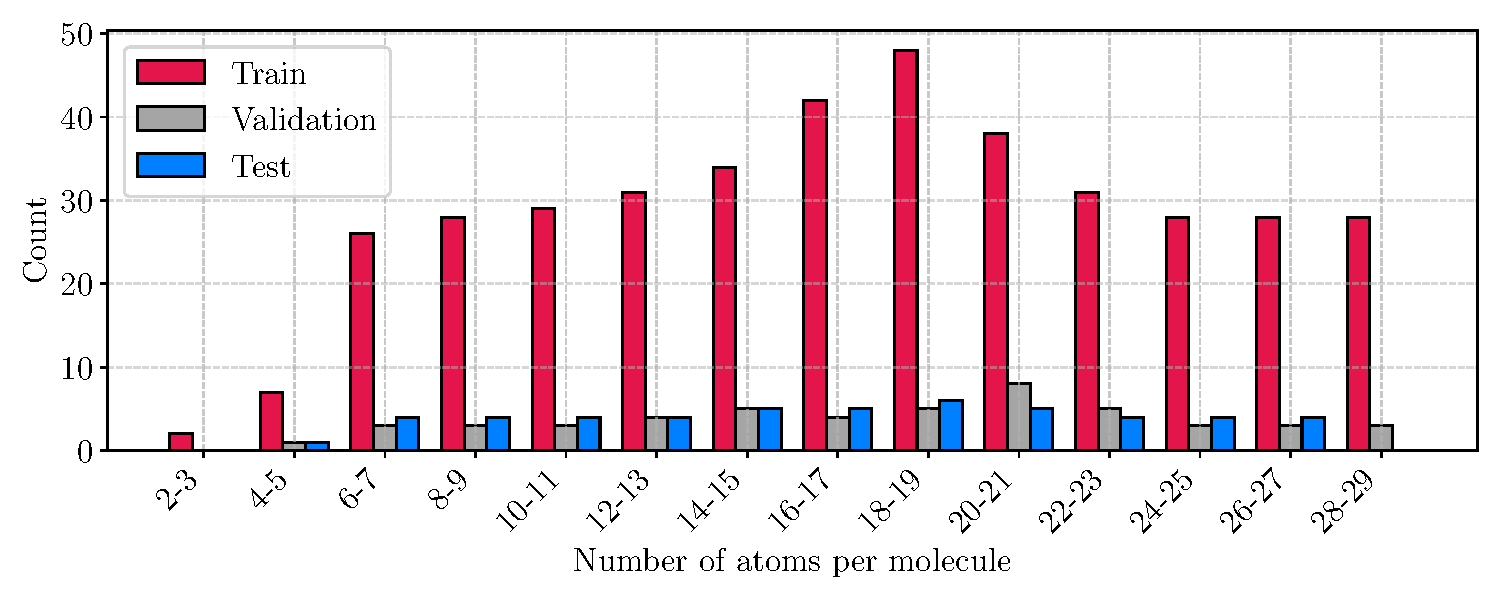
\includegraphics[width=0.85\textwidth]{../fig/application/strat_sample.pdf}
    \caption[Stratified sample of QM9 dataset]{Stratified sample of QM9 dataset by number of atoms per molecule for each set.}
    \label{fig:sample_QM9}
\end{figure}
We sample 500 molecules from the QM9 set in a stratified manner and additionally ensure ample representation for various molecule sizes. Therefore, compared to the actual distribution seen in \autoref{fig:method_qm9_overview}, the representation of molecules with 6 to 13 and 24 to 29 atoms per molecule is increased. This results in the distribution for the train, validation and test sets shown in \autoref{fig:sample_QM9}. Once again the train / validation / test split is 80\% / 10\% / 10\%.

Zero-shot predictions like those devised in the previous section aren't possible on the full dataset due to missing encoders/decoders for \ch{N}, \ch{F} and their respective interaction blocks. Therefore, we'll proceed directly to hyperparameter tuning. 
\subsection{Hyperparameter tuning}
\label{sec:qm9_full_isomers_hyp_tuning}
Network hyperparameter tuning was carried out in the same manner as above, except that the maximum number of training epochs was increased to 50 to accommodate the more diverse dataset. \autoref{tab:qm9_full_further_runs} shows the results for the 10 best performing models.
\begin{table}[H]
    \centering
    \caption[GNN on full QM9 dataset sample with full matrix loss]{GNN on full QM9 dataset sample using full matrix loss and a maximum of 50 epochs to train. Metrics on test set and corresponding hyperparameter settings for 10 best performing networks in terms of iterations.}
    \label{tab:qm9_full_further_runs} 
    \resizebox{\textwidth}{!}{
        \begin{tabular}{l
                        S[table-format=2.1(2)]
                        S[table-format=-4(3)]
                        S[table-format=-1.3(2)]
                        S[table-format=1.3(1)]
                        S[table-format=1.4(1)]}
            \toprule
            Mean metrics:                 & {Iterations / 1} & {$|\Delta E_\text{DFT}|$ / $\unit{\hartree}$}  & {$|\Delta E_\text{DFT}|$ / 1} & {DIIS error / $\unit{\hartree}$} & {RMSE / 1} \\
            \midrule %Data from server run!
            $\text{GNN}^{\text{Full}}_\text{f. 0}$ & 12(2)     & -1070(300) & -0.680(0.04) & 0.20(0.03) & 0.009(0.003) \\ %!TODO not everything rounded good :) 
            $\text{GNN}^{\text{Full}}_\text{f. 1}$ & \textbf{12.0(17)} & -1060(300) & -0.680(0.04) & 0.20(0.03) & \textbf{0.009(2)} \\
            $\text{GNN}^{\text{Full}}_\text{f. 2}$ & 12.0(1.8) & \textbf{-1050(300)} & \textbf{-0.670(4)} & \textbf{0.19(3)} & 0.009(0.003) \\
            $\text{GNN}^{\text{Full}}_\text{f. 3}$ & 12.0(1.9) & -1060(300) & -0.680(0.03) & 0.20(0.03) & 0.009(0.003) \\
            $\text{GNN}^{\text{Full}}_\text{f. 4}$ & 12.0(1.7) & -1060(300) & -0.680(0.04) & 0.20(0.03) & 0.009(0.003) \\
            $\text{GNN}^{\text{Full}}_\text{f. 5}$ & 12.0(1.8) & -1080(300) & -0.680(0.04) & 0.21(0.08) & 0.009(0.003) \\
            $\text{GNN}^{\text{Full}}_\text{f. 6}$ & 12(2)     & -1080(300) & -0.690(0.04) & 0.20(0.03) & 0.009(0.003) \\
            $\text{GNN}^{\text{Full}}_\text{f. 7}$ & 12.1(1.6) & -1080(300) & -0.690(0.04) & 0.20(0.03) & 0.009(0.003) \\
            $\text{GNN}^{\text{Full}}_\text{f. 8}$ & 12(2)     & \textbf{-1050(300)} & \textbf{-0.670(4)} & \textbf{0.19(3)} & 0.009(0.003) \\
            $\text{GNN}^{\text{Full}}_\text{f. 9}$ & 12.1(1.8) & -1090(300) & -0.690(0.04) & 0.21(0.03) & 0.009(0.003) \\
            \bottomrule
        \end{tabular}
    }
        \resizebox{\textwidth}{!}{
        \begin{tabular}{lrrrrrrrrrr}
        \toprule
        Parameters & $\text{GNN}^{\text{Full}}_\text{f. 0}$ & $\text{GNN}^{\text{Full}}_\text{f. 1}$ & $\text{GNN}^{\text{Full}}_\text{f. 2}$ & $\text{GNN}^{\text{Full}}_\text{f. 3}$ & $\text{GNN}^{\text{Full}}_\text{f. 4}$ & $\text{GNN}^{\text{Full}}_\text{f. 5}$ & $\text{GNN}^{\text{Full}}_\text{f. 6}$ & $\text{GNN}^{\text{Full}}_\text{f. 7}$ & $\text{GNN}^{\text{Full}}_\text{f. 8}$ & $\text{GNN}^{\text{Full}}_\text{f. 9}$ \\
        \midrule
        Hidden Dimension & 128 & 256 & 256 & 256 & 512 & 128 & 512 & 512 & 512 & 128 \\
        Batch Size & 8 & 8 & 8 & 8 & 8 & 8 & 8 & 16 & 8 & 8 \\
        Data aug. factor & 4.00 & 1.00 & 1.00 & 1.00 & 1.00 & 2.00 & 4.00 & 3.00 & 1.00 & 2.00 \\
        Edge threshold & 3.40 & 2.58 & 3.98 & 3.21 & 3.29 & 2.85 & 3.27 & 2.72 & 3.44 & 2.30 \\
        Message passing steps & 4 & 5 & 3 & 2 & 4 & 2 & 3 & 3 & 2 & 4 \\
        Message Net Dropout & 0.09 & 0.16 & 0.25 & 0.21 & 0.04 & 0.11 & 0.25 & 0.04 & 0.18 & 0.19 \\
        Message Net Layers & 3 & 3 & 3 & 3 & 3 & 4 & 3 & 2 & 3 & 2 \\
        Learn Rate & 6.90e-04 & 9.31e-04 & 1.61e-03 & 2.75e-04 & 1.51e-04 & 8.03e-04 & 1.26e-04 & 5.85e-04 & 1.09e-03 & 6.50e-04 \\
        Weight Decay & 7.15e-05 & 5.46e-05 & 3.58e-05 & 4.69e-05 & 3.99e-04 & 6.06e-04 & 2.56e-04 & 1.45e-04 & 1.84e-05 & 1.74e-05 \\
        \bottomrule
        \end{tabular}
        }
\end{table}
Both the mean iteration count and its variability increased by about one cycle compared to the best-performing isomer models. Further analysis of iteration performance by molecule size revealed no clear correlation between atom count and the number of iterations to converge.
\subsection{Evaluation \& Conclusion}
\label{sec:qm9_full_isomers_conclusion}
Using our stratified QM9 sample, we show that our GNN implementation trained on just 400 molecules achieves lower SCF iteration counts than every guessing scheme except \text{minao}. The greater chemical diversity in this subset leads to a uniformly higher standard deviation in cycle counts across all methods. \autoref{tab:qm9_full_test_overview} compares our top-performing GNN against the established guessing schemes.

Another notable finding emerges when contrasting the full dataset results for $\overline{P}$ with those from the isomer only runs. Although the average number of iterations remained essentially unchanged (only their spread increased for the more diverse dataset), the DIIS error in the full dataset case is an order of magnitude higher. This increase isn't surprising given the broader chemical variety and the blockwise averaging inherent to $\overline{P}$. Crucially, it once again underscores that DIIS error and iteration count are largely uncorrelated.
\begin{table}[H]
    \centering
    \caption[Models compared to \textsc{PySCF} and $\overline{P}$ schemes - full QM9 dataset]{Comparison of GNN model with calculations employing \textsc{PySCF} and $\overline{P}$ guessing schemes on the full QM9 dataset. Here, $\overline{P}$ is computed blockwise across all molecules by averaging over each \ch{C}, \ch{O}-\ch{H}, \dots\,block.
}
    \label{tab:qm9_full_test_overview}
    \resizebox{\textwidth}{!}{
        \begin{tabular}{l
                        S[table-format=2.1(1.1)]
                        S[table-format=-3.4(3)]
                        S[table-format=-1.6(1.1)]
                        S[table-format=1.3(1.1)]
                        S[table-format=1.4(1.1)]}
                        \toprule
                        Mean metrics:                 & {Iterations / 1} & {$|\Delta E_\text{DFT}|$ / $\unit{\hartree}$}  & {$|\Delta E_\text{DFT}|$ / 1} & {DIIS error / $\unit{\hartree}$} & {RMSE / 1} \\
                        \midrule
                        $\text{GNN}^{\text{Full}}_\text{f. 1}$ & 12.0(17)& -1060(300) & -0.680(0.04) & 0.20(0.03) & \textbf{0.009(2)} \\
                        $\overline{P}$                & 17(3)            & -800(200)  & -0.52(2)     & 0.11(2)   & 0.014(2)  \\
                        \texttt{1-e}                  & 19(3)            & -225(4)    & -0.124(3)    & 0.122(15) & 0.16(12)  \\
                        \texttt{vsap}                 & 14(2)            & -4.8419(4) & -0.002665(19)& \textbf{0.024(3)}  & 0.0106(14)\\
                        \texttt{atom}                 & 16(2)            & -14.0(9)   & -0.0077(5)   & 0.039(7)  & 0.015(2)  \\
                        \texttt{minao}                & \textbf{11.1(11)}& \textbf{2.86(2)} & \textbf{0.001577(0)}& 0.081(12) & 0.017(3)  \\
                        \bottomrule
                    \end{tabular}
    }
\end{table}